%!TEX root = ../report.tex

\section{Object-Oriented Programming}
This chapter explains concepts and terms of object-oriented programming.
The following topics are covered in this chapter:
\begin{itemize}
	\item Foundations of object-oriented programming
	\item Features of object-oriented programming languages
	\item Java and UML syntax
	\item Coupling and Cohesion
	\item Polymorphism
	\item Binding
	\item Delegation
\end{itemize}

\subsection{Foundations of Object-Oriented Programming}
\subsubsection*{Phenomenon and Concept}
Phenomenon is an object in the world of a domain as you perceive it (e.g. watch on your wrist).
Concept describes the common properties of a phenomena (e.g. all watches).
A Concept is a 3-touple of name (e.g. watch), purpose (e.g. measure time) and members (e.g. hourglass, digital watch, ...).

\begin{figure}[h!]
	\centering
	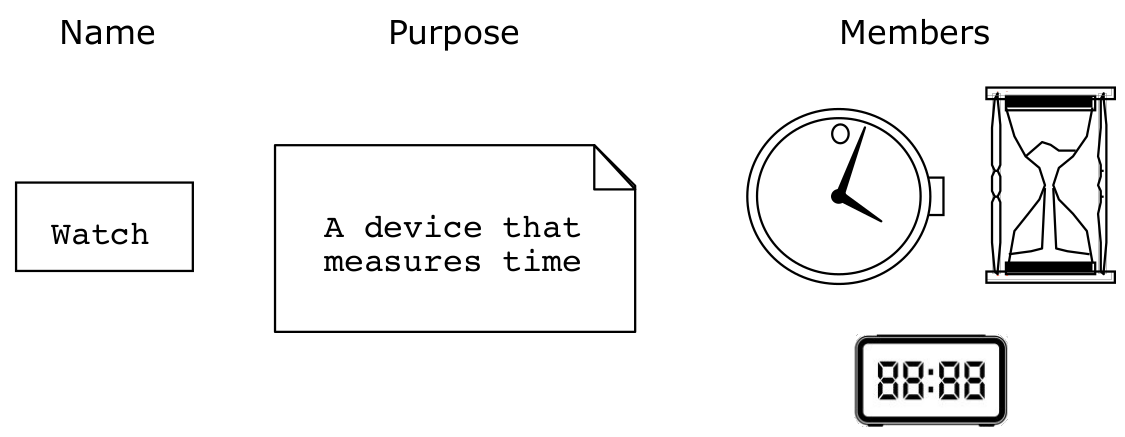
\includegraphics[width=\linewidth]{images/oop_abstraction}
	\caption{Abstraction of Watch}
\end{figure}

\subsubsection*{Abstraction and Modeling}
Abstraction is the classification of a phenomena into concepts.
Modeling is the development of abstractions to answer specific questions about a set of phenomena while ignoring irrelevant details.\newline

\subsubsection*{Type and Instance}
Type is a \textit{concept} in the context of programming languages e.g.:
\begin{center}
	\begin{tabular}{ll}
		\textbf{Name}: int & \textbf{Name}: boolean \\
		\textbf{Purpose}: set of integers & \textbf{Purpose}: logical truth values \\
		\textbf{Members}: 0, -1, 1, 2, -2, \dots & \textbf{Members}: true, false \\
	\end{tabular}
\end{center}

Instance is a member of a specific type.
The type of a variable represents all possible instances of the variable.
Types can be \textit{simple} (primitive) (e.g. int, double, boolean, \dots) or \textit{complex} (e.g. Car, Person, FileSystemService, \dots).

\subsubsection*{Classes and Objects}
In most object-oriented programming languages, a complex type is represented by a class.
A class is a code template for a concept that is used to create instances of that concept.
A class has \textit{attributes (properties)} and \textit{methods (operations)} (e.g. \textit{color} of a car, car can \textit{drive}).
Methods and attributes are called the \textit{members} of a class.\newline

An instance of a class at runtime is called \textit{Object}.


\subsection{Features of object-oriented programming languages}
\subsubsection*{Abstraction}
Creating a model of the problem in terms of classes and the relationships between them.

\subsubsection*{Encapsulation}
Objects are self-contained sets of data and behavior.
By using access modifiers such as \texttt{public}, \texttt{private} or \texttt{protected}, the object can determine which part of its data and behavior is exposed to the outer world.
The exposed parts of an object are called its \textit{public interface}.

\subsubsection*{Information Hiding}
Principle of information hiding (David Parnas):
A calling module (class, subsystem) does not need to know anything about the internals of the called module.
This can be achieved by making all attributes and operations of a class private, unless the operations are needed by the class' user.
Only public methods can be used to modify a class' attributes.

\subsubsection*{Abott's	Heuristics}
This approach analyses natural language to identify objects, attributes and associations from problem descriptions.
\begin{center}
	\begin{tabular}{l|l|l}
		\textbf{Part of speech} & \textbf{Model component} & \textbf{Example} \\
		\hline
		Proper noun & Instance & Alice \\
		Common noun & Class & Field officer \\
		Doing verb & Operation & Creates, submits, selects \\
		Being verb & Inheritance & Is kind of, is one of \\
		Adjective, Genitive case & Attribute & Incident description
	\end{tabular} 
\end{center}
\newpage

\subsection{Java and UML Syntax and Structures}
\begin{figure}[h!]
	\centering
	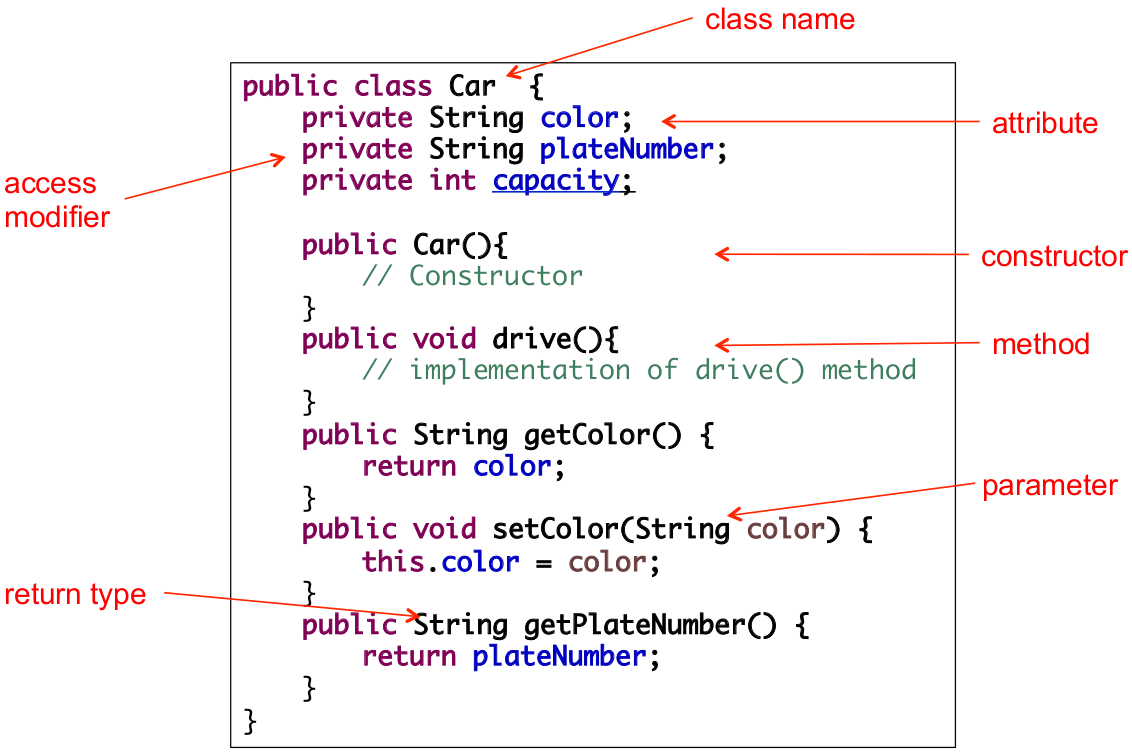
\includegraphics[width=\linewidth]{images/oop_java_class}
	\caption{Java class of \glqq Car\grqq \ and its parts}
\end{figure}

\begin{figure}[h!]
	\centering
	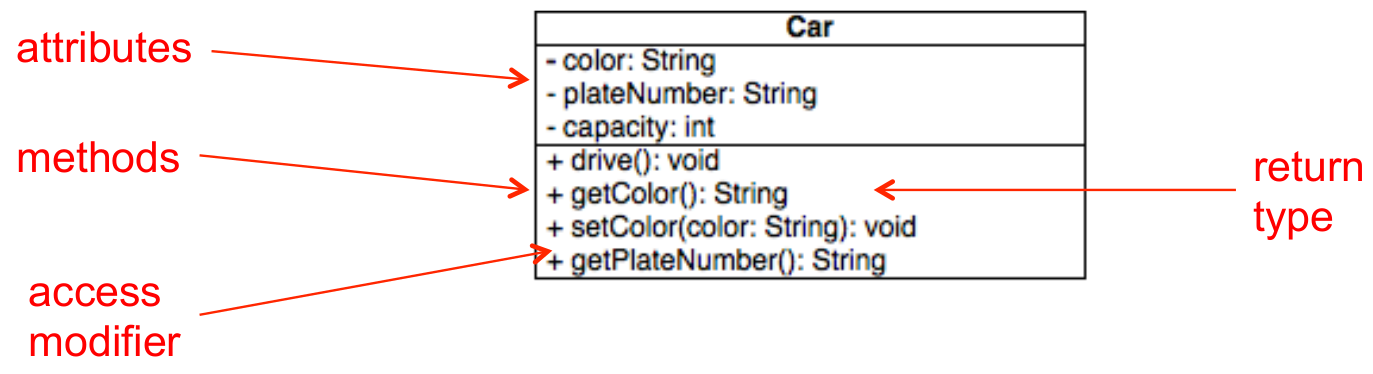
\includegraphics[width=\linewidth]{images/oop_uml_class}
	\caption{UML class diagram of \glqq Car\grqq \ and its parts}
\end{figure}

%TODO? Objects, Static Members, Association, Multiplicity, Aggregation, Composition, Inheritance, Abstract Classes, Interfaces
\subsubsection*{Association/Link}
Represent relationships between classes/objects.
\begin{figure}[H]
	\centering
	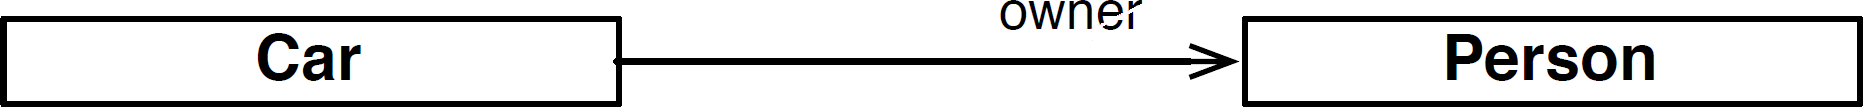
\includegraphics[width=0.85\linewidth]{images/oop_association}
\end{figure}
\subsubsection*{Multiplicity and association names}
Shows the allowed number of links between instances of the classes in an association.\\
Default name for an association end is the name of the connected class.
\begin{figure}[H]
	\centering
	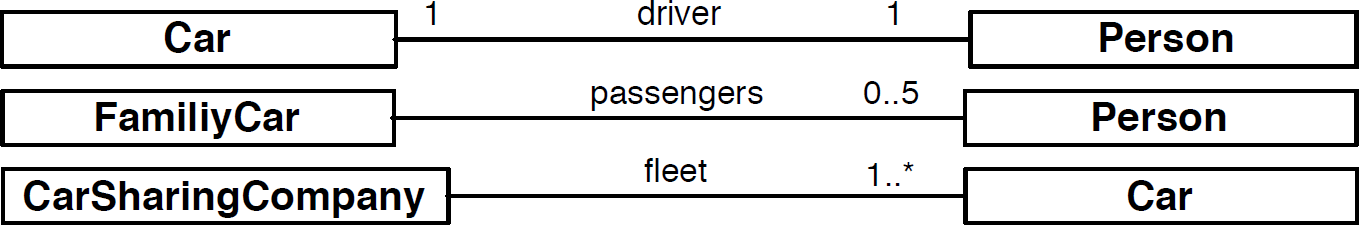
\includegraphics[width=0.85\linewidth]{images/oop_multiplicity}
\end{figure}
\subsubsection*{Aggregation}
Part of, consists of, contains..
\begin{figure}[H]
	\centering
	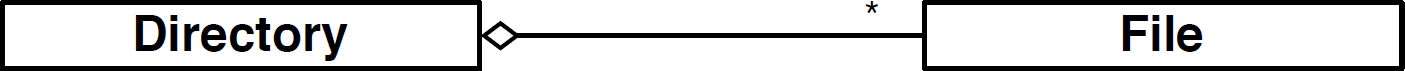
\includegraphics[width=0.85\linewidth]{images/oop_aggregation}
\end{figure}
\subsubsection*{Composition}
Parts cannot exist independent of the composite.
\begin{figure}[H]
	\centering
	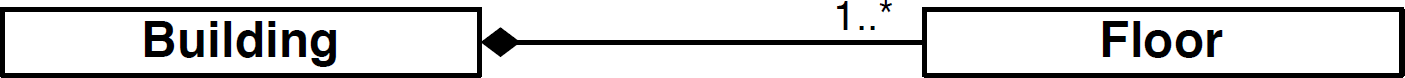
\includegraphics[width=0.85\linewidth]{images/oop_composition}
\end{figure}
\subsubsection*{Inheritance}
\begin{itemize}
	\item Relation between a general class (superclass) and more spezialized class (subclass)
	\item Describes all attributes and operations that are common to a set of classes
	\item Reuse of specification and implementation
\end{itemize}
\begin{figure}[H]
	\centering
	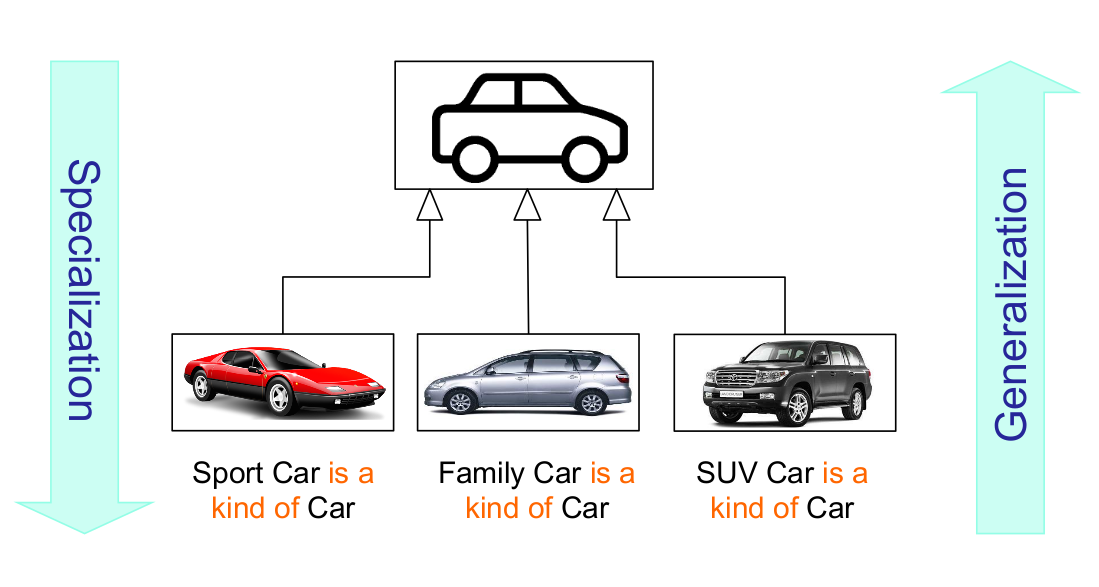
\includegraphics[height=5cm,keepaspectratio]{images/oop_inheritance}
\end{figure}
\subsubsection*{Abstract classes}
Use when a concept is not meant to be instantiated, to model only shared attributes and operations. (Italic letters)
\begin{figure}[H]
	\centering
	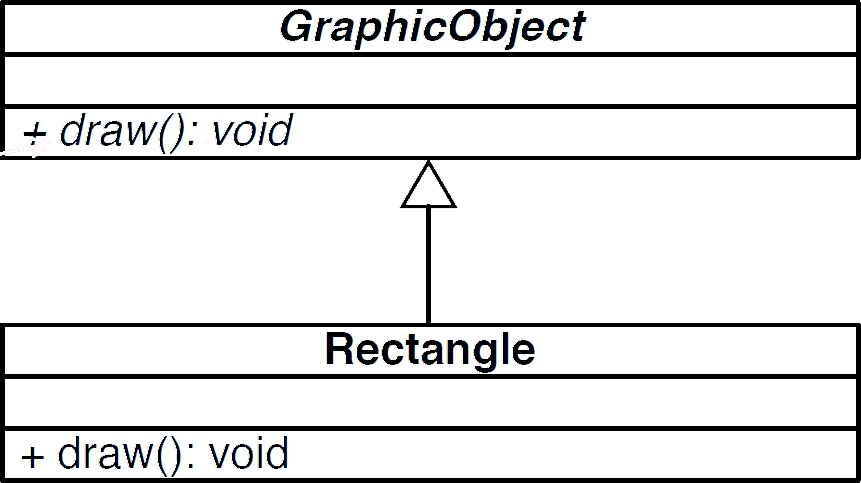
\includegraphics[height=5cm,keepaspectratio]{images/oop_abstract_classes}
\end{figure}
\subsubsection*{Interfaces}
\begin{itemize}
	\item An abstract specification of a types behaviour
	\item Does not contain any implementation of the operations
	\item Formal contract of the bahavior that a class promises to provide
\end{itemize}
\begin{figure}[H]
	\centering
	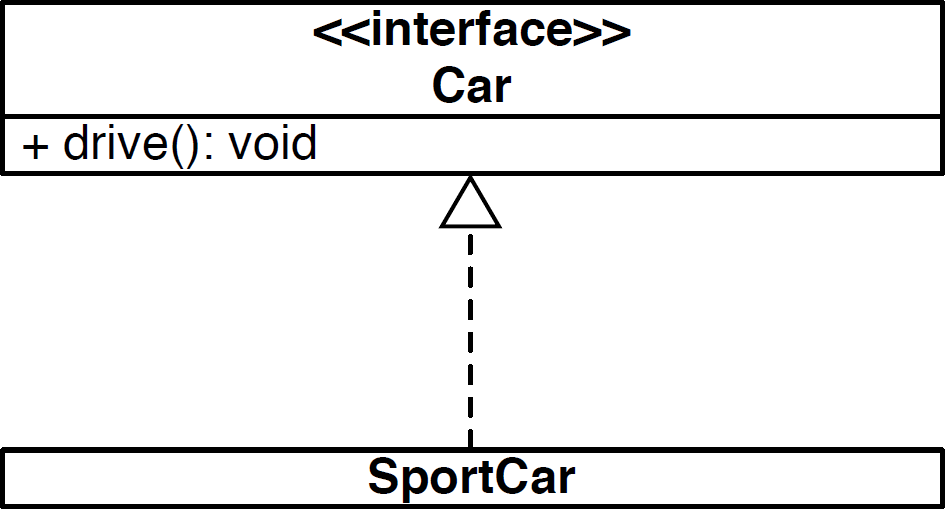
\includegraphics[height=5cm,keepaspectratio]{images/oop_interface}
\end{figure}

\subsection{Coupling and Cohesion}
\textit{Coupling} measures the dependencies between subsystems, \textit{cohesion} the dependencies within a subsystem.
A good design uses low coupling as this makes the subsystem as independent of each other as possible and therefore, changes in one subsystem won't affect other subsystems.
It also uses high cohesion, because subsystems only contain classes which heavily depend on each other.
This approach reduces \textit{complexity} and \textit{eases change} of the system.

To achieve low coupling and high cohesion, the \textit{Principle of Least Knowledge}, also called \textit{Law of Demeter} (Ian Holland) should be followed:

A method M of an object O may only invoke the methods of the following kinds of objects:
\begin{itemize}
	\item O itself
	\item M's parameters
	\item Any objects created/instantiated within M
	\item O's direct component objects
\end{itemize}

In Java, this can be achieved by using only one level of method calls, e.g. \texttt{object.doSomething()}, not two or even more levels e.g. \texttt{object.getObjectP().doSomething()}.
This produces less coupling and is not dependent on implementation details. On the downside, many wrappers may be needed, which can lead to inefficiency.

\begin{figure}[h!]
	\centering
	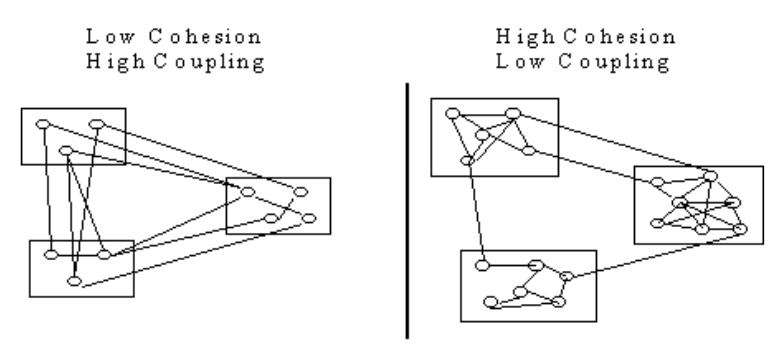
\includegraphics[width=\linewidth]{images/oop_coupling_cohesion}
	\caption{Coupling and Cohesion}
\end{figure}


\subsection{Polymorphism}
Polymorphism is the ability of an object to assume different forms or shapes.
In computer science this is the ability of an abstractions to be realized in multiple ways.
Concretely, this comes down to different ways interfaces can be realized.
Objects can hereby be dynamically treated based on their type.

\subsubsection*{Parametric Polymorphism}
In Java parametric polymorphism can be seen in generic types and operations.
A generic type has a type parameter e.g. \texttt{List<E>}.
A type parameter is a placeholder for a specific type which must be specified at the instantiation of a variable of the generic type.
Operations on generic types are called \textit{generic operations}.

\subsubsection*{Inheritance: Subtyping}
Type A is a subtype of another type B, exactly when all A, considered as a set of values, is a subset of B. B can be substituted by A. This is called Liskov' substitution principle:\newline

\textit{If for each object O\textsubscript{S} of type S there is an object O\textsubscript{T} of type T	such that for all programs P	defined in terms of T, the behavior	of P is unchanged when O\textsubscript{S} is	substituted for O\textsubscript{T}, then S is a subtype of T.}\newline
\begin{flushright}
	--- Barbara Liskov, MIT
\end{flushright}

If a subtype follows the substitution principle, the following rules apply:\newline
\textbf{\textit{Operations:}}
\begin{itemize}[topsep=5pt, itemsep=0pt]
	\item All supertype operations must have corresponding subtype
	operations
	\item Each subtype operation
	\subitem must have a \textit{weaker precondition}: require less (or the	same) than the superclass operation
	\subitem must have a \textit{stronger postcondition}: guarantee more (or the same) than the superclass operation
\end{itemize}
\textbf{\textit{Invariants}} (called properties by Liskov):
\begin{itemize}[topsep=5pt, itemsep=0pt]
	\item Any invariant of the supertype (e.g. value constraints) must be guaranteed by the subtype as well
\end{itemize}

Interfaces and Classes in Java do not guarantee any properties. Therefore, they are not subtypes according to Liskov’s definition.

\subsubsection*{Inheritance: Subclassing}
\textit{Subclassing} denotes the usage of an inheritance association.
\textit{Overriding} is a special case in subclassing where a method implemented in the superclass is reimplemented in the subclass.
The selection of a method depends on the type of the object at runtime.
This allows to change the behavior of an object without extensive case distinctions.

\subsubsection*{Ad-hoc Polymorphism: Overloading}
The ability to let a feature name denote two or more operations is called \textit{overloading}.
Selection of the corresponding methods is decided by the signature.
This decision is made by the compiler.
The signature is defined as the name and parameter types of a method.


\subsection{Binding}
Binding establishes the mapping between names and data objects and their descriptions.

\subsubsection*{Early Binding (Static binding, at compile time)}
The premature choice of operation variant, resulting in possibly wrong results and (in favorable cases) run-time system crashes.

\subsubsection*{Late Binding (Dynamic binding, at run time)}
The guarantee that every execution of an operation will select the correct version of the operation, based on the type of the operation's target.

\subsection{Delegation}
Delegation is a mechanism for code reuse in which an operation resends a message to another class to accomplish the desired behavior.
It involves passing a method call to another object, transforming the input if necessary.
By that, the behavior of an object is extended.

\newpage
